\documentclass[a4paper,12pt]{article}
\usepackage{geometry}
\usepackage{graphicx}
\usepackage{epsfig}
\usepackage{subfigure}
\usepackage{titlesec}
\usepackage{etoolbox}
% Workarounf of stupid bug: http://tex.stackexchange.com/questions/299969/titlesec-loss-of-section-numbering-with-the-new-update-2016-03-15
\makeatletter
\patchcmd{\ttlh@hang}{\parindent\z@}{\parindent\z@\leavevmode}{}{}
\patchcmd{\ttlh@hang}{\noindent}{}{}{}
\makeatother
% --------------------
\usepackage{marginnote}
% \usepackage[round]{natbib}
\usepackage{url}
\usepackage{hyperref}
\usepackage{datetime}
\geometry{tmargin=2.5cm,bmargin=3cm,lmargin=1.5cm,rmargin=1.5cm}
\newcommand{\sectionbreak}{\clearpage}

\begin{document}
\title{QuimP Guide}
\author{Richard Tyson, Till Bretschneider and Piotr Baniukiewicz\\ \small Systems Biology DTC, Warwick University\\ \small Correspondence to Till Bretschneider. Email: \href{mailto:Till.Bretschneider@warwick.ac.uk}{Till.Bretschneider@warwick.ac.uk}\\}
\date{}
\maketitle
\begin{center}
\textbf{{\large Version: 16.08.01-SNAPSHOT}}\\
\vspace{1cm}
Web site: \url{http://go.warwick.ac.uk/quimp}
\vfill
{\footnotesize Manual compiled on \today\  at \currenttime}
\end{center}

\tableofcontents

\setlength{\parskip}{10pt}
\setlength{\parindent}{0pt}

\section{About new QuimP}
%TODO General information about new QuimP, its philosophy and goal

\section{QuimP 16.08.01 - what is new}

\subsection{Summary}
The key features of this version are 
\begin{itemize}
	\item The ability to restore saved BOA state and to continue work from saved point. Module  configuration, plugins settings and current view are saved in the new file format \textit{QCONF}. To maintain backward compatibility, all previously used files are generated as well when exiting BOA. The \textit{QCONF} file is human readable (JSON) and contains all data and parameters generated by BOA. This format is also used by other QuimP modules such as ECMM and Q Analysis. 
	\item New image preprocessing plugins:
	\begin{itemize}
		\item DIC image reconstruction
		\item Random Walker segmentation
		\item Protrusion analysis
	\end{itemize}   
	\item Binary segmentation integrated with BOA module that allows to create outlines (Snakes) directly from binary masks.
\end{itemize}
	
\subsection{Change log}
For changelog check QuimP web page at: \url{https://github.com/CellDynamics/QuimP/wiki/History}.
Current version of the QuimP software as well as history of changes can be viewed directly from the QuimP Bar plugin (Fig. \ref{fig:quimpBar_menu}).
\begin{figure}[ht]
	\centering
	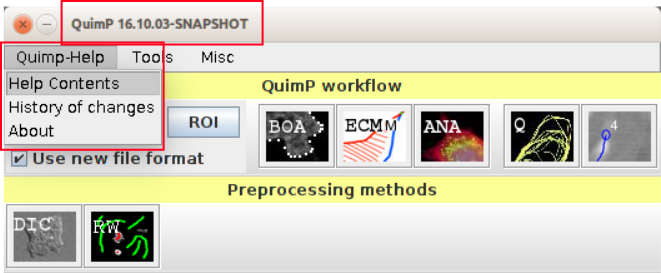
\includegraphics[width=8cm]{quimpBar_menu.png} % requires the graphicx package
	\caption{The QuimP bar}
	\label{fig:quimpBar_menu}
\end{figure}
 	
In case of bugs, contact with QuimP developer: \href{mailto:p.baniukiewicz@warwick.ac.uk}{p.baniukiewicz@warwick.ac.uk}

\section{Installation}

Consult our Wiki page for installation details: \url{https://github.com/CellDynamics/QuimP/wiki/InstallationQuimP}


\section{QuimP Workflow}

There are four stages (and four plugins) to completing an analysis using QuimP.

\begin{enumerate}
	\item Cell segmentation - Performed by the \textbf{BOA} plugin.  Cell outlines, represented as a chain of nodes, are extracted from each frame of an image sequence using an active contour. BOA outputs global measures, such as cell centroid displacement, or cell area.
	\item Membrane tracking - Performed by the \textbf{ECMM Mapping} plugin.  Outlines are mapped between frames to extract local membrane velocities.
	\item Measuring Fluorescence - Performed by the \textbf{ANA} plugin.  Pixel intensities are sampled from the cell's cortex, its width defined by the user.
	\item Data analysis - Performed by the \textbf{Q Analysis} plugin. Statistics are generated and data are visualised in the form of spatial-temporal maps.
\end{enumerate}

Additionally, there are image pre-processing plugins available such as:

\begin{enumerate}
	\item DIC\footnote{Differential Interference Contrast microscopy} plugin (\autoref{sec:DIC})
	\item Random Walker Segmentation plugin (\autoref{sec:RWSeg})
\end{enumerate}

A plugin can be launched from either the $[Plugins\rightarrow QuimP]$ menu, or from the QuimP bar
(opened via $[Plugins\rightarrow QuimP\rightarrow QuimP Bar]$).
Running a plugin will either require an image and/or a QuimP parameter file (with extension \textit{.paQP}) generated by BOA.
Plugins must be executed left to right, although steps can be repeated without re-running previous plugins and fluorescence measuring with ANA can be skipped entirely.

Once complete, data can be analysed in Excel or MATLAB.

\begin{figure}[ht]
   \centering
   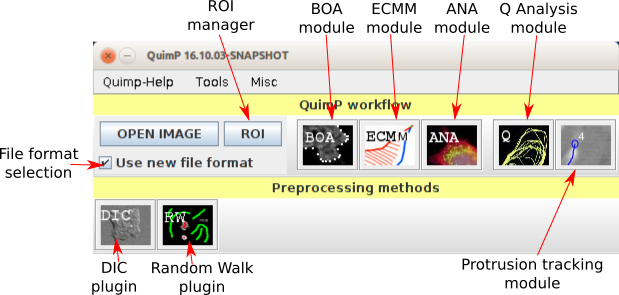
\includegraphics[width=15cm]{quimpBar.png} % requires the graphicx package
   \caption{The QuimP bar}
   \label{quimpBar}
\end{figure}


\section{Cell Segmentation - BOA Plugin}

QuimP utilises an active contour to segment cells from the background of an image.  Typically, this will be a 
time lapse movie containing a fluorescence channel, captured from a confocal microscope, but the BOA plugin will 
segment any image which has bright objects on a dark background (note that phase contrast images can not be 
segmented with this method).  Attaining the best image for segmentation may require some pre-processing, such 
as the combining of available fluorescence channels (the ideal case is that of an evenly white cell on a black 
background).  Figure \ref{activeContour} describes the active contour method and provides insight as to BOA's 
parameters.\\

\begin{figure}[ht]
   \centering
   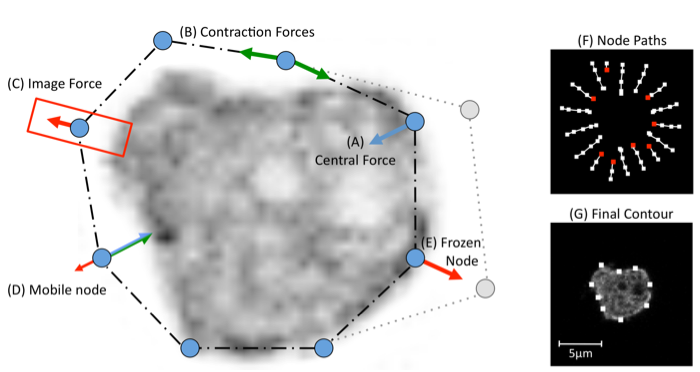
\includegraphics[height=7cm]{activeContour.png} % requires the graphicx package
   \caption{Caricature of outline detection using active
contours.
QuimP's active contour consists of a chain of connected
nodes (a reduced number are shown here for simplicity) initialised
to encircle a cell of interest. Three types of forces act on each
node; (A) Central forces contribute to chain shrinking; (B) Contraction
forces between neighbouring nodes shrink the chain and maintain chain
integrity; (C) Image forces oppose the shrinking of the chain by a
magnitude determined by the local image intensity gradient (red box).
When a node experiences inward forces greater than the opposing
image force it moves inwards (D). On reaching the boundary the image force becomes
sufficiently large to cancel out the other forces, halting and freezing
the node (E). (F) shows the paths of nodes during contraction. Note
that nodes can be added or removed (red nodes) to maintain an average
distance between neighbours. (G) shows the final position of nodes.
QuimP usually makes use of 100 or more nodes to extract high resolution
cell outlines. \cite{Tyson2010}}
   \label{activeContour}
\end{figure}

The BOA window is presented in Figure \ref{boaWindow}. There are \textbf{four} zones that control image segmentation, displaying and postprocessing. 
\begin{itemize}
	\item The red zone contains settings of cell segmentation algorithm, described in \hyperref[step4]{step 4} below. 
	\item The blue zone contains controls for moving across frames in stack and for zooming cells available on current frame.
	\item The green zone contains tools for manual modification of contours.
	\item The yellow zone contains three slots for outline postprocessing filters (described in section \ref{sec:boaFilters})
\end{itemize}

\begin{figure}[ht]
	\centering
	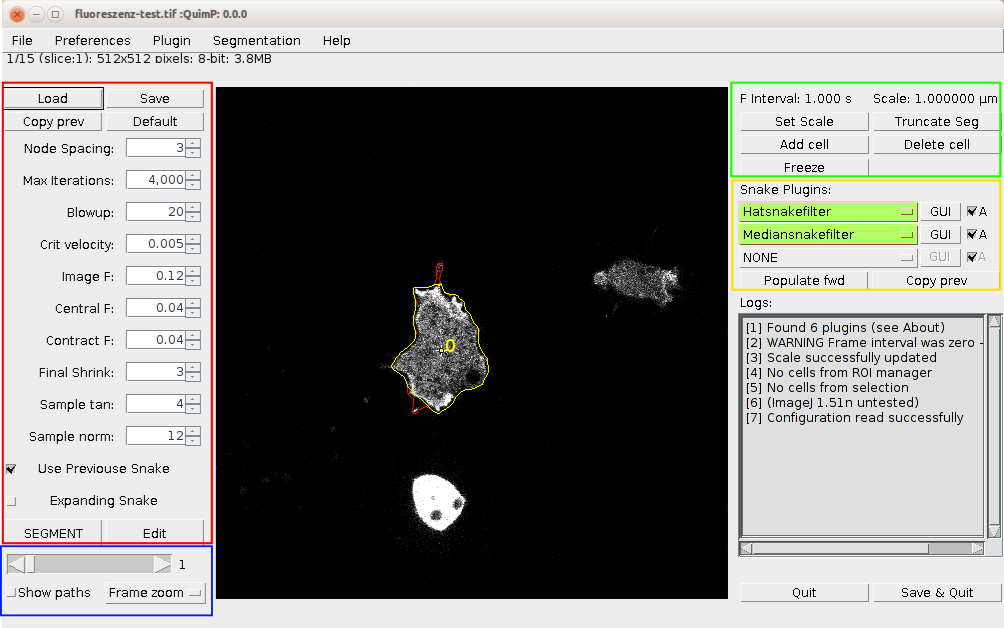
\includegraphics[height=10cm]{boaWindow.png}
	\caption{The BOA Window}
	\label{boaWindow}
\end{figure}
\subsection{BOA menu}
\begin{itemize}
	\item \textbf{File}
	\begin{itemize}
		\item \textit{Load global config} - load \texttt{QCONF} configuration file and restore saved state. One can continue work from point where it was saved in.
		\item \textit{Load plugin preferences} - load configuration of outline plugins stack.  
		\item \textit{Save global preferences} - save configuration of outline plugins stack.
	\end{itemize}
	\item \textbf{Preferences}
	\begin{itemize}
		\item \textit{Plot original} - switch on displaying original outlines together with those processed by plugins. If there is no plugin active (or selected) it does nothing.
		\item \textit{Plot head} - flag zero node of outline with arrow pointing to the outline direction.
		\item \textit{Show history} - open history window.
	\end{itemize}
	\item \hyperref[sec:QuimP_preplugins]{\textbf{Plugin}}
	\begin{itemize}
		\item \textit{Discard all} - remove all plugins from all frames. Discard any change introduced by them to the outline.
		\item \textit{Re-apply all} - try to reload and apply plugins in plugin stack.
	\end{itemize}
	\item \textbf{Segmentation}
	\begin{itemize}
		\item \hyperref[sec:Binary_seg]{\textit{Segment mask}} - perform binary segmentation on black-white mask 
		\item \textit{Clear all} - remove all segmentation results and set all parameters to their default values
	\end{itemize}
	\item \textbf{Help}
	\begin{itemize}
		\item \textit{Help contents} - open system web browser and try to load this manual. Internet connection is required. 
		\item \textit{About} - display version of QuimP and found plugins
	\end{itemize}
\end{itemize}

\subsection{BOA segmentation workflow}
\textbf{Step 1: Open an image and ensure the correct scale.}  QuimP can segment from a single image, or from an image stack
(but not from a hyperstack).  Only 8-bit images can be used for segmentation and so you will be prompted to convert to 8-bit 
if required.  QuimP uses the scale properties of the image to scale all output to
 microns (pixel size) and seconds (frame interval).  \textbf{ENSURE YOUR SCALES ARE CORRECT} within $[Image\rightarrow Properties...]$.
 On launching, BOA will prompt to check your image scale. The scale is recorded by BOA and stored in the parameter file for
 use in the rest of the analysis. 


\textbf{Step 2: Launch the BOA plugin} 

Unlike previous versions, BOA no longer requires selection of cells prior to launching, but you can do so.  Launch BOA from the QuimP bar or menu.
The BOA window is now a fully functional ImageJ window that allows the user to perform any ImageJ function, such as drawing,
creating ROI's, or zooming while the BOA plugin is in use.  Figure \ref{boaWindow} shows the BOA window.
The image scale is displayed at the top right.  To adjust the scale click \textit{Set Scale}.      

BOA can segment one, or more cells, each beginning and ending at any frame you wish.  In addition, you can manually 
edit any segmentation at any frame, add/delete cells, truncate segmentations, and adjust the segmentation
parameters for individual frames.

\textbf{Step 3: Adding and deleting cells.} 

To add a cell first scroll to the frame that you want to begin the segmentation at (either with the mouse wheel, or slider).  Using either the
circular, rectangular or polygon selection tool, draw an ROI (region of interest) around a cell, and click \textit{Add cell}.
BOA will immediately attempt to segment 
the cell at the current frame.  If convergence is successful, the result is displayed as an image overlay. The cell is also given an
identification number.
If the segmentation fails for some reason, the parameters can be adjusted (see below). You do not need to re-add the cell.

Additional cells can be added in the same way.   The active contours surrounding each cell will interact with one another and prevent
contours crossing over to other cells.  This capability is particularly useful in situations where cells come into close contact, 
which often disrupts the segmentation process.

To delete a cell click \textit{Delete cell}, and then click the centre marker of a cell, on any frame where a segmentation is visible.  Hit the same 
button again to leave delete mode.


\textbf{Step 4: Adjusting segmentation parameters.}.\phantomsection\label{step4}  When a parameter is altered, BOA immediately re-computes the segmentation
for all cells on the current frame with the new parameters (all cells share the same parameters).  Each has a minimum/maximum
value that can not be exceeded.  To alter a parameter either enter a value into the text box, or use the arrows to increase/decrease in steps.
First, try adjusting the \textit{Image F} parameter to improve the result.

The parameters are as follows:

\begin{itemize}
\item \textbf{Node spacing} - Roughly equates to the number of pixels between nodes, and hence the resolution of the segmentation.
\item \textbf{Max iterations} - The maximum number of iterations applied to shrink the contour.
\item \textbf{Blowup} - The number of pixels to expand the solution to the previous frame, for beginning 
calculation at the current frame (utilised when `Use previous snake' is active).  Increase if your target cell is moving by large 
amounts between frames.  Decrease if other cells are coming into close proximity and interfering with the snake.  Lower
values reduce computation time.
\item \textbf{Critical velocity} - The cut-off speed at which nodes are frozen.  Lower the value to allow the snake to continue 
to contract for longer, which may aid in letting nodes enter concavities.
\item \textbf{Image F} - Controls the magnitude of the image force pushing nodes outwards.  This is the most effective parameter 
and should be the first port of call for adjustment.  Highly intense cells will produce high image forces, and you may need to lower 
this value to allow nodes to approach the cell outline.  With weakly intense cells the snake may collapse inwards, past the cell 
boundary, in which case increase the image force.
\item \textbf{Central F} - The magnitude of the central force pulling nodes inwards.  Increase to shrink the snake further and help nodes enter concavities.
Decrease to prevent nodes entering the interior of cells. 
\item \textbf{Contract F} - Magnitude of the force pulling nodes together (i.e. contracting the snake).  Increase to prevent nodes `falling
through holes', or to produce a smoother final solution.
\item \textbf{Final shrink} - The number of pixel to shrink the solution to tighten the snake to the cell boundary.  A value of zero does
not shrink the solution at all.
\item \textbf{Sample tan, Sample norm} - Defines (in pixels) the size of the sampling box around each node within which the 
image is sampled for calculation of the image force.  `tan' describes its width, `norm' its depth.  A larger sampling box will increase 
the size of the image force.  Briefly, the sampling box should be an appropriate size as to give an accurate sample of the local
 intensity between the cell and the background.
\item \textbf{Use previous snake} - If selected, the solution to the previous frame will be used as the starting contour for the current frame.
Otherwise, the users selection is used as the starting contour for every frame.
\item \textbf{Expanding snake} - Experimental option. Rather than contract the snake, it expands.  May be useful for tracking vesicles.
\end{itemize}

The key to attaining a good segmentation is the balancing of the 3 forces. Previous segmentations for your image can be loaded
back into BOA by hitting load and selecting a QuimP parameter file with the file extension \textit{.paQP}.
Parameter values alone can be loaded by declining to load associated snakes.

Enabling the tick box labelled \textit{Show paths} will display a trace of the snake as it contracts.  Nodes colour pixels white as they
move towards the cell boundary.  This view can be useful for diagnosing why a segmentation fails.

Enabling the tick box labelled \textit{Zoom cell}, will zoom the image to the first cell added, and track the zoom to 
the cell's movements.


\textbf{Step 5: Segmenting multiple frames.}  When happy with the segmentation on the first frame, hit \textit{SEGMENT} to segment
the cell (or cells) in the following frames.  The algorithm may fail at a particular frame and a warning will be printed to the log window,
at which point you can alter parameters.

\textbf{Step 6: Correcting segmentations.}  In the case of failure, or incorrect results, you have 3 options:

\begin{itemize}
\item \textbf{1 - Edit a solution.} Scroll to a frame where an error occurred, click \textit{EDIT} (If you have more than one cell
click its centre). Drag the points of the ROI to the correct locations (you can hold \textit{alt} to delete nodes or \textit{shift to split nodes}).
You can zoom using the imageJ tool (magnifying glass). If you loose your ROI go to $[Edit\rightarrow selection\rightarrow restore selection]$.
Scroll to edit other frames.  When finished, leave edit mode by clicking \textit{*STOP EDIT*}.
\item \textbf{2 - Adjust the parameters.}  Scroll to a frame where an error occurred and change the parameters to improve the segmentation.
Optionally, click \textit{SEGMENT} to apply these new parameters to the following frames.
\item \textbf{3 - Truncate segmentations.}  Scroll to the first frame where an error occurred and click \textit{Truncate Seg'}.  Click the centre
of a cell to remove all segmentations from the current frame onwards.
\end{itemize}


\textbf{Step 7: Save the results.}  Click \textit{FINISH}.  The saved cell outlines are those visible on the blue overlay.
A set of files will be outputted for each segmented cell.  A cell's ID number is automatically added to filenames.

Enter a name for the analysis (file name extensions are added automatically). BOA outputs files with a \textit{.xxQP} extension.

Files extended  with \textit{.paQP} contain file paths and parameters associated with a particular analysis.  
When running other QuimP plugins, it is the \textit{.paQP} file which you must select to continue an analysis (see \ref{paQP}).

Files extended \textit{.snQP} contain all data associated with individual nodes of an outline, including pixel coordinates, local cortex 
intensity, local membrane velocities, and tracking data (see \ref{snQP}).

Files extended \textit{.stQP.csv} contain average statistics per frame, and can be opened directly in 
Excel as a `comma separated file'  (see \ref{stats}).

The BOA plugin alone outputs many useful statistics regarding cell morphology and migration, without the need to run any further analysis.
Simply open the \textit{.stQP.csv} file in Excel, or use the accompanying scripts to load data into MATLAB (see section \ref{matlab}).

\subsection{Filtering the outline}
\label{sec:boaFilters}
%TODO Finish Filtering the outline

\subsection{A Few Words on Image Segmentation}

If you run into difficulties attaining a good segmentation, there are a few tricks that may help.  If the width of your cell is around 20 pixels or less
try artificially increasing the size of the image with some form of pixel interpolation selected ($[Image \rightarrow Adjust \rightarrow Size]$).
This should aid sampling of the image and allow nodes to enter concavities with greater ease (note, all subsequent analysis
must be performed on the image at the new resolution).

If your images are particular noisy, and cell's appear very grainy, you may try applying a weak Gaussian blur to smooth them
($[Process\rightarrow Filters\rightarrow Gaussian Blur]$).  This should make for more reliable sampling of the cell's interior.

Remember to recalculate the scale of the image when resizing, and to perform intensity analysis on the rescaled image without any interpolation.

Another common approach to improving image quality is to remove background noise using a `blank' image, one taken without any
cells in the field.  This is particularly useful for removing shadows of dirt on the optical equipment, and correcting uneven backgrounds.

\subsection{Binary segmentation} \label{sec:Binary_seg}
The QuimP supports creation of Snake outlines directly from binary masks. As the active contour method is not used in this case, one can use another segmentation algorithms (e.g. \hyperref[sec:RWSeg]{Random Walker method}) to deal with problems that typically occur for active contour such as e.g. bad segmentation of cavities.

To use binary segmentation, the black-white mask (8-bit image in ImageJ) should be prepared first. It has to be size of segmented image that is already loaded to BOA plugin. The number of slices in mask file should be less or equal to the number of slices present in segmented image. \textbf{The background pixels must have value 0 whereas objects can be defined by any other values within the range 1-255}.

The binary segmentation plugin can be launched from BOA menu $(\textit{Segmentation}\rightarrow \textit{Binary segmentation})$

\begin{figure}[hp]
	\centering
	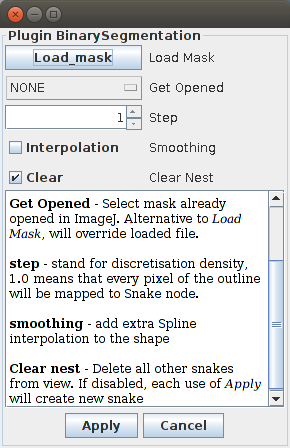
\includegraphics[height=10cm]{BinarySeg.png}
	\caption{The Binary Segmentation Window}
	\label{BinarySegWindow}
\end{figure}

The mask can be either loaded from separate file (ImageJ formats are supported) or selected among already opened images in ImageJ. Results of segmentation are displayed in real-time on BOA window immediately after clicking \textit{Apply}. \textit{Cancel} closes the plugin window leaving last results of segmentation in BOA.    
 
\section{Cell Tracking - ECMM Plugin}

To extract data on local membrane velocity QuimP utilises our Electrostatic Contour Migration Method (ECMM).  
Nodes that form a cell outline at time \textit{t} are mapped onto the segmented outline at time \textit{t+1}.  The distance a node migrates
during the mapping process, and the frame interval, determines the local membrane velocity at the node's position.  If you only have a single
frame there is no need to run this plugin.  ECMM edits and adds to data 
already contained within an \textit{.snQP} file.

\textbf{Step 1: Launch the ECMM Mapping plugin, and open the desired \textit{.paQP} file when prompted.}  There are no parameters that
require manual setting.

\textbf{Step 2: Inspect the results}.  The blue outline represents the cell outline at time $t$, the green at time $t+1$.  
Green circles, overlaid with crosses, denote intersection points that have been validated and used for calculating sectors.  
Red lines denote paths taken by migrated nodes.   Nodes that fail to map correctly are highlighted in yellow.
Failed~node (FN) warnings are displayed along with a running total (in brackets) of the number of failed nodes in the whole sequence.  
The log window will display progress and warnings. 

If a node fails to map it is simply ignored, the effect of this is a small reduction in mapping resolution at the nodes location.
If the process fails to map the majority of the nodes correctly, then a new segmentation will have to be performed
(try using a different node resolution or changing the image resolution).

\subsection{ECMM Tracking}
\label{ecmmTracking}

The details as to the workings of ECMM can be found in our publication \cite{Tyson2010}.
The current implementation includes several significant improvements.  It is not necessary to understand the method,
only the format of the tracking.

At frame $t=1$ a node is randomly chosen as being node zero, $n_{0}$.  Other nodes are then assigned a position
according to their distance from $n_{0}$ along the cell perimeter.  The length of the cell perimeter 
is normalised to $1$, hence the position of a node which is exactly half way around the perimeter will be 0.5
(see figure \ref{ecmm}a).

\begin{figure}[ht]
   \centering
   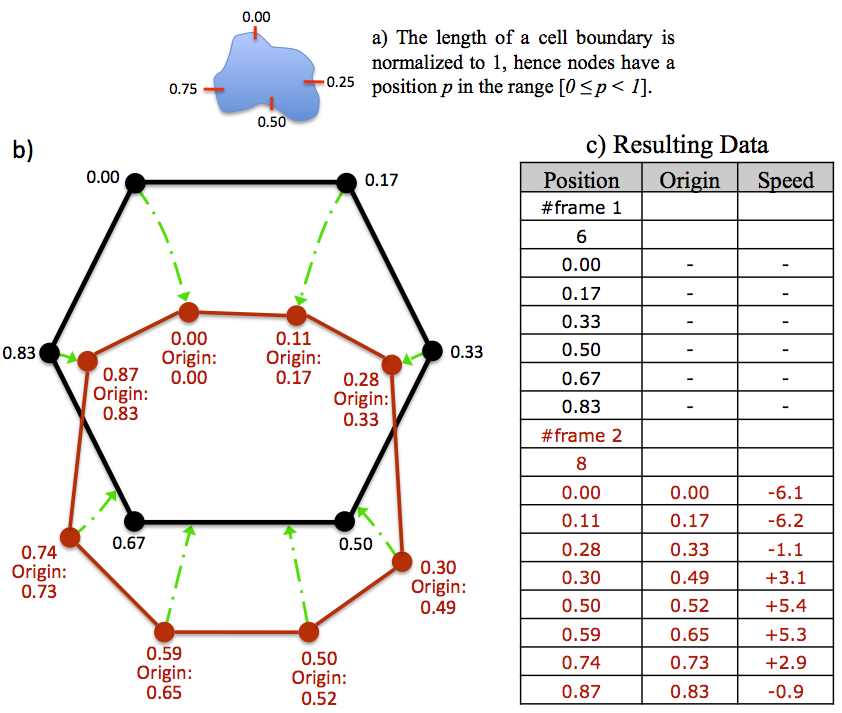
\includegraphics[height=10cm]{ecmm.png}
   \caption{\textbf{ECMM tracking method. a)} Normalisation of the cell perimeter. \textbf{b)} Caricature of the tracking of node positions
   between two frames (black $t$, red $t+1$). Arrows pointing towards the red outline indicate forward mappings and a nodes origin is recorded simply
   as its position on the black outline. Arrows pointing towards the black outline indicate reverse mapping and node origins
   are recorded as interpolated values between nodes on the back outline.
    \textbf{c)} Data from \textit{b)} as it would appear in a \textit{.snQP} file. The frame number is followed by the number of nodes in the outline.
    Speeds are proportional to the lengths of the green mapping arrows.}
   \label{ecmm}
\end{figure}


The nodes of the outline at $t=2$ also have positions assigned, but in addition have an \textit{origin}.  This represents 
where a node originated from on the $t=1$ outline.  For example, a node with an origin of 0.5 originated from 
position 0.5, exactly half way around the outline at $t=1$.

It should be realised that this method of tracking is sub-node resolution.  By simply interpolating the positions and origins of 
nodes, any real number position on an outline can be tracked at sub-node resolution, for as many frames as desired.  See section
\ref{snQP} for the format of data output, and section \ref{trackingMaps} for using ECMM data within MATLAB.


\section{Fluorescence Measurements - ANA Plugin}
\label{ana}

QuimP samples the intensity of pixels from within the cortical region of a cell.  At each frame, nodes of the cell outline
are shrunk inwards to form an inner outline.  The amount of shrinkage is specified by the user, and relates to the
estimated cortex width.  Nodes are 
migrated inwards towards the inner outline, while simultaneously measuring pixel intensities  (a 3x3 average).  
A nodes fluorescence intensity is the maximum recorded as it migrates across the cortex.  ANA can record data for up to 3 separate 
fluorescence channels.

\begin{figure}[ht]
   \centering
   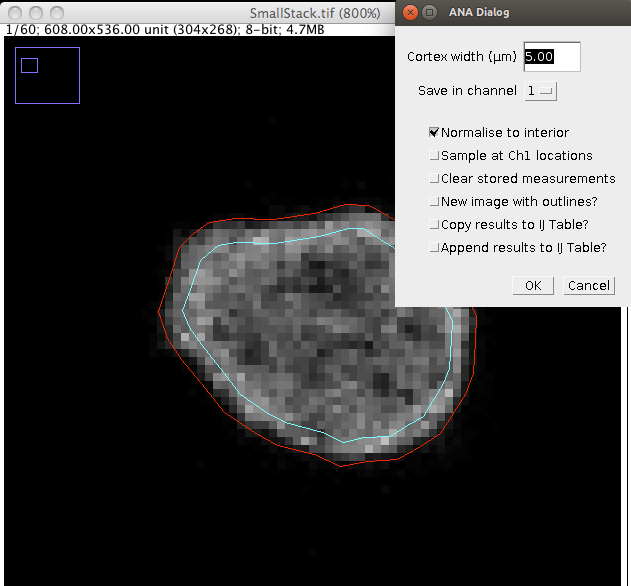
\includegraphics[height=8cm]{ana.png} % requires the graphicx package
   \caption{ANA.  The area between the red and blue contours is the user defined cortex, and is where
   intensity samples are taken. If \emph{Normalise to interior} is ticked, sampled intensities will be normalised
   to the average intensity of pixels within the blue contour.}
   \label{fig:ana}
\end{figure}

\textbf{Step 1: Open an image stack containing the desired fluorescence channel.}  This may be the same stack used 
for cell segmentation, or one containing data from another channel.  Ensure the opened stack has the 
same resolution and number of frames as that used for segmentation.

\textbf{Step 2: Launch the ANA plugin and open the desired \textit{.paQP} or (recommended) \textit{QCONF} file when prompted.}

\textbf{Step 3: Enter a value for the cortex width ($\mu m$) and choose a channel.}  The inner and outer outlines
are displayed on the image.  Changing the cortex width will update the image overlay.
Choose a channel to record data in from the drop down menu.

ANA provides 3 further options
\begin{itemize}
	\item Normalise to interior - Toggle normalisation of intensity sampling to the cells interior (recommended).
	\item Sample at Ch1 locations - Sample at the same locations as determined for channel 1.
	\item Clear stored measurements - Removal all fluorescence measurements from QuimP's files.
\end{itemize}

Click \textit{OK}.
  
Fluorescence data associated with specific nodes is added to either \textit{.snQP} 
file and the \textit{QCONF} file, while whole cell data (e.g. total cortex fluorescence) is written to the \textit{.stQP.csv} file.

\textbf{Step 4: For further channels, open the next channel image and re-run ANA.}

\section{Compiling Data - Q Analysis Plugin}

Data within \textit{.snQP} and \textit{.stQP} files can be read into Matlab at this point, but motility maps have not yet been generated.
The Q Analysis plugin will build spatial-temporal maps of motility, fluorescence, and convexity,
and also several other maps to aid analysis.  In addition, vector graphics are produced 
using the \textit{Scalable Vector Graphics} format.  These include a cell track in which all cell outlines are overlaid and coloured
according to frame number, and a motility movie in which nodes are coloured with a user specified data type.

\textbf{Step 1: Launch the Q Analysis plugin and open the desired \textit{.paQP} file when prompted}.

\begin{figure}[ht]
   \centering
   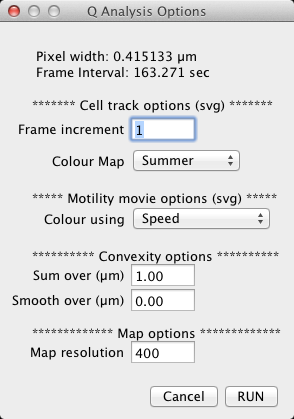
\includegraphics[height=10cm]{screenQAnalysis.png} 
   \caption{Q Analysis options dialog}
   \label{screenQAnalysis}
\end{figure}

\textbf{Step 2: Enter parameters to the options dialog}.  The parameters are as follows:

\begin{itemize}

\item \textbf{Cell track option - Frame increment}  [positive integer].  The frame increment for drawing the
cell track (\textit{\_track.svg}).  Frames are only draw at the specified increment.  Set to 1 for all frames.  
\item \textbf{Cell track option - Colour Map}.  Select a colour scheme for the cell track.
\item \textbf{Motility movie option - Colour using.}. Select the data type for use in colouring nodes of the motility movie.
\item \textbf{Convexity option - Sum over (microns)} [positive real number].  Distance around the cell 
perimeter ($\mu m$) to sum curvature. Set to zero for no summation.
\item \textbf{Convexity option - Smooth over (microns)} [positive real number].  Distance around the cell 
perimeter ($\mu m$) to over which to average curvature for smoothing. Set to zero for no smoothing.
\item \textbf{Map option - Map resolution} [positive integer]. A value of $x$ will produce images that are
$X$ pixels in width.  The height of the image will be equal to the number of frames of the analysed sequence,
or a multiple of number of frames (if less then $x$). Data is interpolated to form maps of any size.
\end{itemize}

The images produced are for visualisation only, as they have been scaled to fill the RGB colour spectrum.
Vertical image scale is set to frames (frame zero at the top),
horizontal to the normalised length of the cell perimeter (0,1].
Import $.maQP$ files as text images for further analysis in ImageJ. See Section~\ref{maps} for details
and analysis of maps.

\section{QuimP preprocessing plugins}
\label{sec:QuimP_preplugins}
\subsection{DIC images processing}
\label{sec:DIC}

Differential interference contrast microscopy (DIC) enhances the contrast in unstained, transparent samples. DIC images can be easily interpreted and analyzed by biologists due to high resolution available and excellent contrast generated by steep gradients in optical path lengths and phase shifts between the two polarized beams. Nevertheless, very characteristic bas-relief observed in DIC images is the source of problems in automatic analysis of these images. The image contrast and the same the object’s boundaries are well defined in the shear angle but in direction perpendicular to it there is no contrast against to background and thus a lack of distinct edges of object. Moreover, strong gradient of image intensity at shear angle negatively influence standard image processing methods like global thresholding or edge detection producing insufficient results, with discontinuous regions or edges.

The DIC plugin provided with QuimP allows to convert DIC samples into form more suitable for segmentation and further image processing. The local contract for any cell in reconstructed image is well defined in every direction and the intensities of pixels take only positive values (in relation to a mean intensity level). The algorithm implemented in QuimP is described in \cite{Kam1998}. Either single images or time lapse movies from DIC microscopy can be processed. 

\textbf{Step 1: Open an image.}
Once loaded into ImageJ/Fiji click DIC filter in QuimP bar. Only 8-bits images are supported (256 gray levels).

\textbf{Step 2: Set correct parameters}
There are two important parameters: \textit{Shear} angle and \textit{Decay} (Fig. \ref{fig:dicdialog}). The \textit{Shear} parameter is the shear angle of DIC microscopy measured anticlockwise, whereas \textit{Decay} is described in details at \cite{Kam1998}. The value of \textit{Decay} depends mainly on the size of cells and the best results are achieved experimentally. 
   
\begin{figure}[ht]
	\centering
	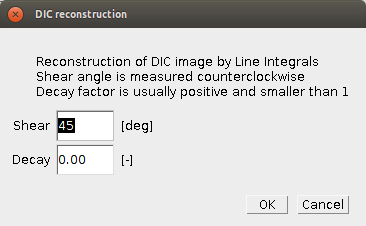
\includegraphics[width=10cm]{DICwindow.png} 
	\caption{DIC filter options dialog}
	\label{fig:dicdialog}
\end{figure} 

\subsection{Random Walker Segmentation}
\label{sec:RWSeg}

The Random Walks Segmentation algorithm is described in the paper \cite{Grady2006}. It belongs to the class of supervised segmentation algorithms what means that the user interaction is needed. In RW method a user has to specify a small set of pixels belonging to the desired object and
(possibly) a set of pixels belonging to the background. Those pixels are called seed pixels and in this plugin they form the seed image. The seed image must be the size of segmented image whereas, the number of layers can be equal or smaller than in segmented image. The RW plugin can be called outside of QuimP directly from the QuimP Bar. The main interface is presented in figure \ref{fig:rwdialog}.

\begin{figure}[ht]
	\centering
	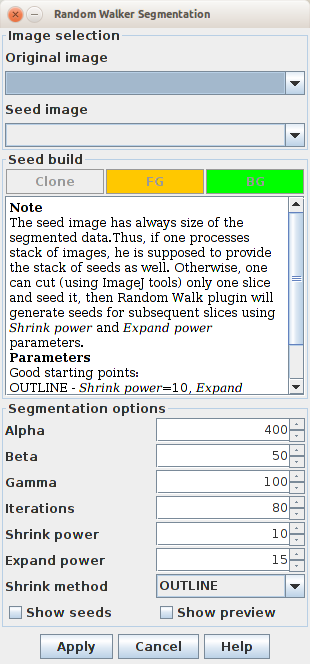
\includegraphics[width=8cm]{screenRandomWalk.png} 
	\caption{Random Walker segmentation dialog}
	\label{fig:rwdialog}
\end{figure}

\subsubsection{Random Walker Segmentation Workflow}

The Random Walker plugin can be used with Binary Segmentation (\ref{sec:Binary_seg}) plugin available in BOA for creation of Snake outlines. Possible workflow is presented below:

\begin{enumerate}
	\item Open \textit{original image} that will be analysed
	\item Open QuimP bar and select RW plugin
	\item Choose \textit{original image} in \textbf{original image} selector
	\item Click \textbf{Clone} to duplicate \textit{original image} and convert it to RGB format
	\item Use \textbf{BG} and \textbf{FG} buttons to select background pen and foreground pen respectively. Use these pens for scribbling background and objects.
	\item Set parameters - default are usually ok and click \textbf{Apply}. Segmented image will be shown.
	\item Select \textit{original image} and start BOA from QuimP bar
	\item Consult binary segmentation plugin documentation \ref{sec:Binary_seg} how to use your segmented image for generating BOA outlines   
\end{enumerate}

\subsection{Protrusion tracking}
\label{sec:PtrotTracking}

%TODO Finish Protrusion tracking
 
\section{Data Files Explained}

\subsection{Parameter files - new format vs. old format}
The latest QuimP introduces a new file format support\footnote{above QuimP11}. The \textit{QCONF} file is based on human-readable JSON format and it is designed to hold all results evaluated by QuimP on every stage of data processing, together with configuration parameters, algorithm settings, etc. 
Initially, the \textit{QCONF} is generated by BOA plugin together with standard \textit{paQP} and \textit{snQP} files. Then, it can be loaded and saved by every other QuimP module. The \textit{QCONF} is not replacement for "old" formats - it rather extends them and allows for easy sharing of results between different QuimP modules, restoring work from last point and keeping the whole QuimP configuration in one place.   

Currently, QuimP understands both formats, but its behavior depends on which format is loaded to module:
\begin{itemize}
	\item loading \textit{QCONF} file to QuimP module causes that this file will be updated and saved back. Files in previous format (\textit{paQP}, \textit{snQP}, etc) will be generated as well and saved in the same directory. \textbf{This is recommended approach.}
	\item loading \textit{paQP} to QuimP module switches QuimP to compatibility mode - all files in previous formats will be generated in the same way as QuimP11, \textit{QCONF} will not be generated or updated. 
\end{itemize}     
Note that when operating with QCONF files, QuimP modules can overwrite existing \textit{paQP} and \textit{snQP} files. The content of those files do not change but the file creation date does. Relations between module and file are summarized in Table \ref{filestable}. Legend for Table \ref{filestable} is as follows:
\begin{itemize}
	\item \textbf{N} - file is created.
	\item \textbf{M} - file is modified - new data are appended to it.
	\item \textbf{C} - file is changed - some data are replaced.
\end{itemize}

The \textit{QCONF} file can be loaded to Matlab using one of the free JSON parsers (tested with JSONlab\footnote{\url{http://uk.mathworks.com/matlabcentral/fileexchange/33381-jsonlab--a-toolbox-to-encode-decode-json-files}}).
\begin{table}[]
	\centering
	\caption{Relation among modules and generated files}
	\label{filestable}
	\begin{tabular}{|l|l|l|l|l|l|l|l|l|}
		&  \textbf{paQP}&  \textbf{snQP}&  \textbf{maQP}&  \textbf{stQP.csv}&  \textbf{QCONF}&  \textbf{pgQP}& \textbf{svg}&  \textbf{tiff}\\ \hline
		\textbf{BOA} &   N&  N&  &  N&  N&  N&  &  \\
		\textbf{ECMM}&    &  C&  &   &  M&   &  &  \\
		\textbf{ANA} &   M&  M&  &  M&  M&   &  &  \\
		\textbf{Q Analysis}&  &  &  N&  &  M&  &  N& N 
	\end{tabular}
\end{table}

  
\subsection{Parameter Files - \textit{paQP} Files}
\label{paQP}

A parameter file contains text and has the extension \textit{.paQP}.  Both QuimP's plugins and
MATLAB functions use the parameter file to locate files associated with an analysis and also to store data such as the
pixel size, frame interval, and start frame.  In addition, it stores the parameters used for segmentation
(the last used parameters).

The first line identifies the file as a QuimP parameter file, and contains the creation date.
The second is random identifier.
The third is the absolute path to the image used for segmentation.
 
In general, the contents of a parameter file should not be changed, but you may wish to alter the paths to
image files if you later move them.
 

\subsection{Snake Data - snQP files}
\label{snQP}

The \textit{.snQP} file contains data relating to the nodes of cell outlines (\textit{snake} is a reference to active contours being 
described as snakes).   Comment lines
begin with a \#.  Data for frame $f$ begins with the comment line \textit{\#frame f}, followed by a single integer value
indicating the number of nodes that make up the outline ($N$).  The following $N$ rows hold the data for the nodes. The 
columns are as follows:

\begin{itemize}

\item \textbf{Node Position} - The normalised position of the node in relation
to node zero, $n_{0}$ (see section \ref{ecmmTracking}).

\item \textbf{X\_coord} - The horizontal pixel coordinate of a node on the image used for segmentation.

\item  \textbf{Y\_coord} - The vertical pixel coordinate of a node on the image used for segmentation.

\item \textbf{Origin} - The position from which a node originated from on the outline
at the previous frame (see section \ref{ecmmTracking}).

\item \textbf{Global Origin} - The position from which a node originated from on the outline
at the first segmented frame (see section \ref{ecmmTracking}).

\item \textbf{Speed} [microns per second]- The speed at which a node travelled between frames, as determined by ECMM.

\item \textbf{Fluor\_Ch\$} - The intensity value assigned to a node by ANA (see section \ref{ana}) for the channel
number denoted by \$.  This value is the maximal $3x3$ average intensity measured at the node's local cortical region.

\item \textbf{Ch\$\_x} - The horizontal pixel co-ordinate on the fluorescence image at the point where Fluor\_Ch\$ was measured, i.e.
the co-ordinate where the maximum intensity occurred.

\item \textbf{Ch\$\_y} - The vertical pixel co-ordinate on the fluorescence image at the point where Fluor\_Ch\$ was measured, i.e.
the co-ordinate where the maximum intensity occurred.

It is possible to store data for 3 fluorescence channels ($\$=\{1,2,3\}$) within the \textit{.snQP} file. Missing 
data is denoted by negative values.

\end{itemize}

\subsection{Frame statistics - stQP files}
\label{stats}

The statistics file, with the extension \textit{.stQP}, contains whole cell statistics for each frame (rather than node associated
data).  Data is written as \textit{comma separated values} which can be opened easily as a spreadsheet.  The file is split into
two section.  Data in the top section is computed by BOA and relates to cell morphology and movement of the cell centroid.
Data in the lower section relates to cell fluorescence and was computed
by ANA (data is listed separately for all 3 available channels). Missing data is denoted by $-1$.

The cell centroid is computed as the weighted centre of the polygon formed by the cell outline.
The measures computed by BOA are as follows:


\begin{itemize}

	\item \textbf{X-Centroid} [$pixels$] - Horizontal pixel co-ordinate of the cell centroid.

	\item \textbf{Y-Centroid} [$pixels$] - Vertical pixel co-ordinate of the cell centroid.
	
	\item \textbf{Displacement} [$microns$] - Distance the cell centroid has moved from its position in the first recorded frame. 
	
	\item \textbf{Distance Travelled} [$microns$] - Sum of the centroid displacements between frame, i.e. the total distance 
	over which the centroid has moved.
	
	\item \textbf{Directionality} - Persistence in direction, calculated as $Displacement / Dist. Travelled$ (chemotaxis index). A value of 1 reveals that
	a cell has moved in a straight line.  Decreasing values denote a cell moving increasingly erratically.
	
	\item \textbf{Speed} [$microns~per~second$] - Speed at which the centroid moved between the current and previous frame.
	
	 \item \textbf{Perimeter} [$microns$] - Length of the cell perimeter (segmented outline).
	  
	 \item \textbf{Elongation} - An ellipse is fitted to the cell outline and the major/minor axis used to compute the elongation of 
	 the cell's shape. $Elongation = major~axis / minor~axis$. Note that a value of 1 does not necessarily represent
	 a perfectly circular cell, only a circular fitted ellipse.
	 
	 \item \textbf{Circularity}  - A measure of circularity defined by the following equation:
	$\frac{4*PI*Area}{Perimeter^{2}}$. A value of 1 reveals the cell's outline to be perfectly circular.
	 
	 \item \textbf{Area} [$microns^{2}$] - Cell area.
	 
\end{itemize}

The measures computed by ANA are as follows:

\begin{itemize}

	\item \textbf{Total fluo.} [$pixel intensity$] - Total fluorescence. Sum of all pixel intensities within the cell outline. 

	\item \textbf{Mean fluo.} [$pixels intensity$] -  Mean fluorescence. Average intensity of pixels within the cell outline.

	\item \textbf{Cortex width} [$microns$] - Width of the cortex, as specified by the user (see section \ref{ana}).
	
	\item \textbf{Cyto. area} [$microns^{2}$] - Area of the cytoplasm (area of the whole cell minus the cortex area).
	
	\item \textbf{Total cyto. fluo.} [$pixels~intensity$] - Sum of all pixel intensities within the cytoplasm. 
	
	\item \textbf{Mean cyto. fluo.} [$pixels~intensity$] - Average pixel intensity within the cytoplasm.
	
	\item \textbf{Cortex area} [$microns^{2}$] - Area of the cortex.
	
	\item \textbf{Total cortex fluo.} [$pixels~intensity$] - Sum of all pixel intensities within the cortex. 
	
	\item \textbf{Mean cortex fluo.} [$pixels~intensity$] - Average pixel intensity within the cortex.
	
\end{itemize}


\subsection{QuimP Maps - maQP files}
\label{maps}

The images produced by Q Analysis are spatial-temporal maps of motility, convexity, and fluorescence.  The vertical axis represents 
time, with frame 1 at the top.  The horizontal axis represents positions along the cell outline, the length of which
has been normalised to 1 at every frame.  Outlines can be
thought of as having been `cut' at position zero, laid along the horizontal axis, and stacked below one another, hence maps
are cylindrical (wrap around onto themselves on the horizontal axis). 

The node randomly designated as begin node zero ($n^0$), at frame 1, is mapped to the top left
pixel.  Data from ECMM is used to track the position of $n^0$
throughout all the frames, and is always positioned at the left most pixel at each frame.  All other nodes are positioned along 
the horizontal axis according to their distance from $n^0$ 
along the cell perimeter.  Values between nodes are estimated using linear interpolation. 

If the number of frames is below the specified map resolution, then maps are scaled vertically, hence 
a row of pixels may be an interpolated value between frames.  

As well as producing \textit{.tif} images, maps are also 
saved as text images with the extension \textit{.maPQ}.  Unlike the \textit{.tif} maps, these are not scaled vertically, so each line of 
values contains the data for a single frame.  It is these maps that should be used for further analysis.

Similarly, four additional maps are produced to aid further analysis:

\begin{itemize}

\item \textbf{Motility Map.}   Pixels are coloured according to node speed, as calculated by ECMM.  Red shades 
represent expanding regions, blue shades contracting regions.  Pixel values
within the \textit{tiff} image are scaled to fill the colour spectrum.  The map file extended \textit{\_motilityMap.maPQ} contains 
un-scaled values, in \textit{microns per second}. 

\item \textbf{Fluorescence Maps}.  A fluorescence map is produced for each channel that data has been 
recorded into.  The fluorescence map images display pixel intensities, as extracted by the ANA plugin.
Files extended \textit{\_fluoCh\$.maPQ} contain the respective data. 

\item \textbf{Convexity Map}.   Represents the curvature of the cell, measured in the range $[-1,1)$, where negative values are concave (blue),
and positive convex (red).
As with the motility map, values
are scaled to fill the colour map. Files extended \textit{\_convexityMap.maPQ} contain the respective data (un-scaled). 

\item \textbf{Co-ordinate Map (a.k.a. Position Map)}.  As described in section \ref{ecmmTracking}, each node has an
associated position.  The co-ordinate map, rather than contain values regarding
motility, fluorescence or convexity, instead contains the position values of nodes.  The main
purpose of the co-ordinate map, along with the origin map, is for tracking positions through time (see section \ref{trackingMaps}).

\item \textbf{Origin Map}. As described in section \ref{ecmmTracking}, each node has an origin, the position a node originated from
on the previous frame.  The origin map contains origin values and can be used, along
with the co-ordinate map, to track positions through time (see section \ref{trackingMaps}).

\item \textbf{xMap}.  Contains horizontal image pixel co-ordinates (those on the image used for segmentation) relating to map pixels.

\item \textbf{yMap}.  Contains vertical image pixel co-ordinates (those on the image used for segmentation) relating to map pixels.

\end{itemize}


\subsection{Scalable vector graphics output - svg files}

Files extended with
\textit{.svg} can be viewed natively in most internet browsers (Windows Explorer requires the Adobe SVG viewer), or opened and edited
in graphics software ( e.g. Inkscape, free software for mac).  The 
Scalable Vector Graphics (svg) file format can be viewed at any desired resolution. 

\begin{itemize}

\item \textbf{Cell track}.  An overlay of all cell outlines coloured according to frame number. Files extension \textit{\_track.svg}.

\item \textbf{Cell motility movie}.  Data contained within the motility/fluorescence/convexity map is displayed on the cell track. Extension \textit{\_motility.svg}.

\end{itemize}

\subsection{BOA plugins stack configuration - pgQP file}

This file stores configuration of plugin stack together with configurations of active plugins (see Figure \ref{boaWindow} and chapter \ref{sec:boaFilters}). This file is not related to any loaded data therefore it can be exchanged between projects. Complex plugin stack configuration is stored also in \textit{QCONF} file. 

%\section{Tracing paths through frames}

%This section will describes methods for tracking positions through time. See section \ref{trackingMaps}.

\section{MATLAB Functions}
\label{matlab}

QuimP outputs a large amount of data for each cell analysed.
You may want to write custom scripts for analysis, but we provide
a set of MATLAB functions to remove the hassle of loading/organising data, and performing
simple operations, such as plotting maps.
We hope to make data as accessible and as explorable as possible to allow adaptation to a users specific goals.

Help documentation is included with each function which can be accessed in the
usual way by typing \textit{help functionName} at
the MATLAB command prompt.  At the end of this document is a walkthrough analysis using the provided test images
(see section \ref{walkthrough}).

\subsection{Loading data - \textit{readQanalysis.m}  }

The first step is to launch the script \textit{readQanalysis.m} which handles loading of data from multiple
cells.  Given a directory, it will search that directory, and all sub-directories, for \textit{.paQP} files. For each parameter file
that is found an analysis structure is built.  As data is read from sub-directories, you may organise your separate analyses into 
sub-directories, but placing all files into the same directory is still possible. Missing files are skipped, hence it is not necessary
to have run all the QuimP plugins.


Loading data relies on the maintenance
of file names imposed by the QuimP plugins, and requires associated files to
be present in the same directory as the parameter file.
The exceptions to this are the images used for segmentation and fluorescence measurements.  Paths to these images are
stored in full to allow separation of analysis files from image data.  If images are moved, and subsequently cannot
be located, the directory where the parameter file is stored will be searched.  You may edit the \textit{.paQP} file to alter
paths to the images if you wish
(note that images are not loaded into memory by \textit{readQanalysis.m}, instead the function checks only that they exist
and sets a path to them).

The output of \textit{readQanalysis.m} is an array of structures, $C$, each element holding data for a single analysed cell.
The contents of an analysis structure is as follows ($F$ = number of frames, $N^{f}$ = number of nodes at frame $f$):

\begin{itemize}

 \item \textbf{name} [$string$] - File name element common to all associated files (name of the parameter file).
 
  \item \textbf{index} [$integer$] - Cell ID, in order read in.
 
 \item \textbf{PATH} [$string$] - Directory of the parameter file.
 
 \item \textbf{\$FILE} [$string$] - Filenames of  QuimP output.
 
 \item \textbf{\$TIFF} [$string$] - Filenames of an image sequences.
 
  \item \textbf{outlines} [$cell~array~(F\times1)$]  - Holds node associated data. Each element
 contains a matrix of size $N^{f}\times6$,
each row being a node. Column headers are [Position , X-coord , Y-coord , Origin , Global origin ,  Speed].
 
 \item \textbf{outlineHeaders} [$cell~array~(1\times6)$] - Descriptions of column measures within \textit{outlines},
  as stated above.
  
 \item \textbf{fluo} [$cell~array~(F\times1)$] - Holds node fluorescence data for all three channels. Each element contains a 
  3D matrix of size $N^{f}\times3\times3$.  The first dimension represents nodes, second the channel number, and third the
  measure.   The measures are [Intensity , X-coord , Y-coord], where the x and y co-ordinates provide the location of
  sampling (see section \ref{ana}).  For example, the intensity sampled at node 23, on channel 2 is located at (23,2,1).
  
 \item \textbf{fluoHeaders} [$cell~array~(1\times3)$] - Descriptions of measures within \textit{fluo}, as 
 stated above.
 
 \item \textbf{nbFrames} [$integer$] - The number of frames.

 \item \textbf{startFrame} [$integer$] - The first frame segmented relative to the the image used for segmentation.

 \item \textbf{endFrame} [$integer$] - The last frame segmented relative to the the image used for segmentation.

 \item \textbf{frames} [$vector~(F\times1)$] - Vector of the segmented frames relative to the the image used for segmentation.
 
  \item \textbf{PixelSize} [$double$] - Pixel size in microns (image scale).

 \item \textbf{frameInterval} [$double$] - Frame interval in seconds.
  
 \item \textbf{R} [$vector~(1\times4)$] - Pixel co-ordinates of a bounding box encompassing all movement of the cell.
 R = [x min, x max, y min, y max]. 
 
  \item \textbf{maxSpeed} [$vector~(F\times1)$] - For each frame the maximum node speed is calculated.
  This is useful for scaling plots.

 \item \textbf{stats} [$matrix~(F\times11)$] - Holds whole cell statistics relating to the cell centroid and cell shape (see
 section \ref{stats}).  Rows contain data for frames.  The column headers are ['Frame'    'x-Centroid'    'Y-Centroid' 
 'Displacement'   'Distance Travelled'    'Directionality'  'Speed'    'Perimeter'    'Elongation'    'Circularity'    'Area']

  \item \textbf{statsHeaders} [$cell~array~(1\times11)$] - Descriptions of column measure within \textit{stats}, as stated above.
  
  \item \textbf{fluoStats} [$matrix~(F\times3\times11)$] - Holds global cell statistics relating to the cell fluorescence (as described in
 section \ref{stats}).  The first dimension is frame number,  second the channel number, and third the measure.  The 
 measure headers are ['Frame'    'Total Fluo.'    'Mean Fluo.'    'Cortex Width'    'Cyto. Area'    'Total Cyto. Fluo.'
  'Mean Cyto. Fluo.'    'Cortex Area'    'Total Cortex Fluo.'    'Mean Cortex Fluo.'    '\%age Cortex Fluo.'].  Missing data is represented
  by negative values, typically $-1$.
  
  \item \textbf{fluoStatHeaders} [$cell~array~(1\times3)$] - Descriptions of the measures in the third dimensional
  within \textit{fluo}, as stated above.
  
  \item \textbf{cortexWidth} [$vector~(3\times1)$] - Holds for each channel the cortex width specified when running ANA. 
  
   \item \textbf{$\ast$Map} [$matrix~(F\times MapRes)$] - Maps read from \textit{.maQP} files (see section \ref{maps}).  A QuimP map 
   in MATLAB is a 2D matrix, rows being frames, columns being discrete points along the cell outline.

  \item \textbf{forwardMap} - see section \ref{trackingMaps}.
  
  \item \textbf{backwardMap} - see section \ref{trackingMaps}.
     
\end{itemize}


\subsection{Function Overview}

Functions prefixed with `read'  are used by \textit{readQanalysis.m} and so generally are not used
independently, but can be if desired.    For details of usage please refer to the
functions help by typing \textit{help functionName} at the MATLAB command prompt.

\begin{itemize}

 \item \textbf{buildTrackMaps} - Constructs the \textit{forwardMap} and \textit{backwardMap} based 
 upon the co-ordinate and origin maps.  These are used to track through QuimP maps.  See section \ref{trackingMaps} for details.
 
 \item \textbf{mapLookup} - Extract values from maps by specifying a window or region.  This can be used, for example, to extract data
 along tracked paths.
 
 \item \textbf{plotMap} - Plot a QuimP map using specified colour map limits.
 
 \item \textbf{plotMotility} - Plots a cell outline with nodes coloured according to their speed of movement.
 
 \item \textbf{plotOutline} - Plots a cell outline.
 
 \item \textbf{trackBackwards} - Utilises the \textit{backwardMap} to track backwards through a map, from a specified point,
 in accordance with the ECMM tracking data. 
 
 \item \textbf{trackForwards} - Utilises the \textit{forwardMap} to track forwards through a map, from a specified point,
 in accordance with the ECMM tracking data.
 
  \item \textbf{trackForwAcc} - Similar to \textit{trackForwards} but functions at sub-pixel resolution. More accurate but slower.
   
 \item \textbf{xcorrQ} - Perform cross-correlation and auto-correlation of .maPQ maps.
 
 \end{itemize}

\subsection{Tracking Maps}
\label{trackingMaps}

The term \textit{tracking} in this sense refers to being able to pick a position on the perimeter of a cell and identify its corresponding
position in the following frames, and hence, track a position over time.  The trace of a position, computed by ECMM,
can be plotted on top of a QuimP map. 

A QuimP map in MATLAB is a 2D matrix, rows being frames ($f$) and columns being discrete locations along the cell outline ($l$).
An incorrect view may be that a map pixel $p$ at frame $f$, and location $l$, ($p^{f}_{l}$),  tracks to the pixel directly 
below ($p^{f+1}_{l}$).  This is not the case,
$p^{f+1}_{l}$ does not necessarily originate from $p^{f}_{l}$.  The origin map must be consulted to identify the
correct location.

[Maps that enforce $p^{f}_{l}$ tracking to $p^{f+1}_{l}$ become heavily distorted, and certain regions lose
resolution severely.]

To track from $p^{f}_{l}$ to $p^{f+1}_{l2}$ we require the correct matrix column index at $f+1$, $l2$.  Firstly, 
consult the co-ordinate map at $p^{f}_{l}$ to identify the position on the cell outline.  Next, extract
the values in row $f+1$ from the origin map.  The index $l2$ is simply the index of the closest origin value to $p^{f}_{l}$'s position
(this can also be done at sub-pixel resolution for more accuracy).
The process is repeated to find $p^{f+2}_{l3}$, $p^{f+3}_{l4}$, etc.  In a similar way, positions can be tracked backwards in time.

This tracking procedure is implemented in the provided MATLAB functions. The function \textit{buildTrackMaps.m} creates
two additional maps, \textit{forwardMap} and \textit{backwardMap}, and is called when data is read in.
An element in the \textit{forwardMap}, for example at $p^{f}_{l}$, contains the correct column index for $l2$ to
locate $p^{f+1}_{l2}$.  Similarly, \textit{backwardMap} contains the correct values for finding $p^{f-1}$.

Functions \textit{trackForwards.m}, \textit{trackForwAcc.m} and \textit{trackBackwards.m}, given a frame, location,
and number of frames to track over, will return complete traces for you.
Consult the help for these functions for details of usage and the walkthrough for an example.


\section{Walkthrough analysis}
\label{walkthrough}

The folder \emph{QuimP\_walkthrough\_files} contains 3 tiff image sequences which you can
analyse (images are courtesy of Evgeny Zatulovskiy, Rob Kay Group, MRC Laboratory of Molecular Biology).

\begin{itemize}
	\item `QW\_channel\_1\_actin.tif'- Actin label.  Image and has been background corrected and contrast enhanced.
	\item `QW\_channel\_2\_neg.tif' - Negative stain.  The cell appears as a shadow on a bright
	background, which has then been inverted.
	\item `QW\_channel\_2\_seg.tif' - For segmentation we shall use the negative stain channel.  
	A 1~pixel Gaussian blur has been applied, the background removed, and contrast enhanced.  
\end{itemize}

\textbf{Step 1}. Open ImageJ and launch the QuimP bar $[Plugins\rightarrow QuimP\rightarrow QuimP Bar]$.  Open the image `QW\_channel\_2\_seg.tif'.  Launch BOA from the QuimP bar.

\textbf{Step 2}. At the prompt check the scale is correct (2 second frame interval, pixel width 0.2 microns).

\textbf{Step 3}. Using the polygon selection tool, create a selection encompassing the cell. This can be very rough.
Click \emph{Add cell}.

\textbf{Step 4}.  Adjust the parameters to get a good segmentation.  Click \emph{SEGMENT} and wait for completion.

\textbf{Step 5}. Scroll through the sequence to check the segmentation result using either the scroll bar or mouse
wheel. The segmentation should have completed to the last frame.  If not, we will truncate the segmentation.
Scroll to the last frame which successfully segmented and click \emph{Truncate Seg}.
Click \emph{FINISH}, and provide a name for the analysis (e.g. `QTest').

\textbf{Step 6}. Launch the ECMM plugin from the QuimP bar. It does not require an image. When prompted,
locate the QuimP parameter file you just created (e.g QTest.paQP).  ECMM will run.
You can view the result and close the image.

\textbf{Step 7}. Open the image 'QW\_channel\_1\_actin.tif'.  With it in focus, launch the ANA plugin,
and again select your parameter file.  Choose a sensible cortex width (e.g. 1.5 microns).
Make sure `save in channel' is set to 1, and normalise to interior is ticked.  Click \emph{ok}.
When complete, ANA will show the sample locations for the last frame.

\textbf{Step 8}. Close 'QW\_channel\_1\_actin.tif', and open `QW\_channel\_2\_neg.tif'.  We will record another
channel for good measure.  Repeat the last step, but with the channel 2 image, this time storing
data in channel 2 (which is the default), and tick 'Sample at Ch1 locations'.  ANA will now
use the same sample points as computed for channel 1 (useful if you want to compute ratios between channels).

\textbf{Step 9}. Launch the Q Analysis plugin, and again choose your parameter file. Check your scale is what you expect at the top of the parameter window. We will use all the
current defaults, so click \emph{RUN}.  Inspect your maps, all of which are automatically saved to disk.

\textbf{Step 10}. The displayed images have been scaled to cover the colour space. The raw values have been saved
separately as text files, with the extension \emph{.maQP} (e.g.  QTest\_0\_fluoCh1.maQP).
You can view them in ImageJ by opening them via $[File -> Import -> Text Image...]$.

\textbf{Step 11} We will now switch to MATLAB to plot some of this data.  Open MATALB
and open the script file 'walkthrough.m', which will guide you through loading and plotting data.
You can use the output provided in the QuimP package, called \textit{QWalkthrough}, rather than
your own.

\section {Historical versions}

\subsection{QuimP11b}

\begin{enumerate}
	\item Fixed several minor bugs.
	\item Updated and tested with ImageJ 1.49a and MATLAB 2014a
	\item The ECMM and Q Analysis plugins will search for other .paQP in a directory and prompt to batch process files.
	\item BOA prompts to check image scale.
	\item BOA can read in a previous segmentation using the LOAD button
	\item When editing segmentations the user can scroll between frames without leaving edit mode
\end{enumerate}

\section{Contact}

The QuimP software is being developed at the Systems Biology DTC at the University Of Warwick by the Till Bretschneider group (\textit{Till.Bretschneider@warwick.ac.uk}).
Further information, and future releases, can be obtained from \url{http://go.warwick.ac.uk/quimp}.

QuimP is under continuous development and feedback will be much appreciated.  If you discover a bug, have suggestions 
for features, or simply find a spelling mistake, please contact the developer Piotr Baniukiewicz at \textit{p.baniukiewicz@warwick.ac.uk}. Thank you for supporting our software. 
\bibliographystyle{plain}
\bibliography{references} 
\end{document}


















